\documentclass[a4paper,UTF8]{article}
\usepackage{ctex}
\usepackage[margin=1.25in]{geometry}
\usepackage{color}
\usepackage{graphicx}
\usepackage{amssymb}
\usepackage{amsmath}
\usepackage{amsthm}
%\usepackage[thmmarks, amsmath, thref]{ntheorem}
\theoremstyle{definition}
\newtheorem*{solution}{Solution}
\newtheorem*{prove}{Proof}
\usepackage{multirow}
\usepackage{url}
\usepackage{enumerate}
\usepackage{algorithm}
\usepackage{algorithmic}
\usepackage{mathrsfs}
\renewcommand{\algorithmicrequire}{\textbf{Input:}}
\renewcommand{\algorithmicensure}{\textbf{Procedure:}}
\renewcommand\refname{参考文献}

%--

%--
\begin{document}
\title{实验2. 隐马尔科夫模型实践}
\author{MG1733079,杨佩成,\url{18362903155@163.com}}
\maketitle

\section*{综述}
	隐藏马尔科夫模型(Hidden Markov Model)是一种著名的有向图模型,主要用于时序数据建模,在语音识别、自然语言处理等领域有广泛应用。
\begin{figure}[h]
\centering
\small
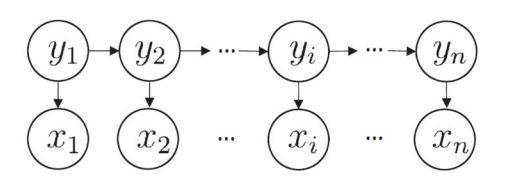
\includegraphics{1.JPG}
\caption{隐马尔科夫模型的图结构}
\end{figure}

	如Figure 1所示,隐马尔科夫模型中的变量可分为两组。第一组是状态变量 $\left\{ y_1,y_2,...,y_n\right\}$,其中$y_i \in \mathcal{Y}$表示第i时刻的系统状态。通常状态变量是隐藏的、不可被观测的,因此状态变量也叫隐变量。第二组是观测变量$\left\{ x_1,x_2,...,x_3 \right\}$,其中$x_i \in \mathcal{X}$表示第i时刻的观测值。
	
	Figure 1中的箭头表示了变量间的依赖关系。在任意时刻,观测变量仅依赖于状态变量。同时,$t$时刻的状态$y_t$仅依赖于$t-1$时刻的状态$y_{t-1}$。基于这种依赖关系,所有变量的联合概率分布为
\begin{displaymath}
	P(x_1,y_1,...,x_n,y_n)=P(y_1)P(x_1|y_1)\prod_{i=2}^nP(y_i|y_{i-1})P(x_i|y_i).
\end{displaymath}

	除了结构信息,要确定一个隐马尔科夫模型需要以下三组参数:
\begin{itemize}
\item
	状态转移概率:模型在各个状态间转换的概率,通常记为矩阵$\textbf{A}=[a_{ij}]_{N\times N}$,其中
\begin{displaymath}
	a_{ij}=P(y_{t+1}=s_j|y_t=s_i),\qquad 1 \leq i,j \leq N,
\end{displaymath}
表示在任意时刻$t$,若状态为$s_i$,则下一时刻状态为$s_j$的概率。
\item
	输出观测概率:模型根据当前状态获得各个观测值的概率,通常记为矩阵$\textbf{B}=[b_{ij}]_{N\times M}$,其中
\begin{displaymath}
	b_{ij}=P(x_t=o_j|y_t=s_i),\qquad 1 \leq i \leq N, 1\leq j \leq M
\end{displaymath}
表示在任意时刻$t$,若状态为$s_i$,则观测值$o_j$被观测的概率。
\item
     初始状态概率:模型在初始时刻各个状态出现的概率,通常记为$\boldsymbol{\pi}=(\pi_1,\pi_2,...,\pi_N)$,其中
\begin{displaymath}
	\pi_i=P(y_1=s_i),\qquad 1\leq i \leq N
\end{displaymath}
表示模型的初始状态为$s_i$的概率。
\end{itemize}

	通过指定状态空间$\mathcal{Y}$、观测空间$\mathcal{X}$和上述三组参数,就可以确定一个隐马尔科夫模型。在本次实验中,我们使用HMM对股票数据进行分析和预测。对于单只股票,我们可以观察到的值可以是涨、跌、不涨不跌。我们假设股票的涨跌由内在的隐变量驱动,即牛市或熊市。

\section*{实验一.}
	实验一我们对训练好的HMM,利用维特比算法对模型进行推断。维特比算法是一种使用动态规划思想来寻找最有可能的隐状态序列的算法,
\begin{algorithm}
	\begin{algorithmic}
		\Require 输入
		\Ensure 输出
		\Function{VITERBI}{$array$}
			\For{$each state i \in \left\{ 1,2,...K \right\}$}
				\State $asd$
			\EndFor
		\EndFunction
	\end{algorithmic}
\end{algorithm}

\section*{实验二.}
	\dots

\section*{实验三. }
	\dots

\end{document}